\section{统计学习导论部分}
    Instructor: Sheng Yu

    In this course, some key formulations/theorem in machine learning are deduced, together with core principles illustrated.

\begin{point}
    What is Machine Learning?
\end{point}

\begin{quote}
    Machine learning is a field of computer science that uses statistical techniques to give computer systems the ability to "learn" with data, without being explicitly programmed.
\end{quote}

Examples of Machine Learning:
    \begin{itemize}[topsep=2pt,itemsep=0pt]
        \item Linear/Logistic Regression (Linear Model)
        \item Decision Tree
        \item Support Vector Machine
        \item Clustering
        \item Bayesian Network
        \item Neural Network
        \item Conditional Random Field
        \item etc.
\end{itemize}

    This section will cover some of the methods above in a machine learning perspective.

\subsection{Linear Model}
    Linear model is the basic model in statistics, see \autoref{SecLinearRegressionAnalysis}. 

\subsubsection{Linear Model in Machine Learning Perspective}
    In machine learning field, key feature of linear model is its affine form of variable dependence:
    \[
        Y=f(X)+\varepsilon = \tilde{f}_\beta (X'\beta )+\varepsilon  
    \]

    where usually $ X=(1,X_{1},X_{2},\ldots,X_{p}) $, $ \beta =(\beta _0,\beta _{1},\beta _{2},\ldots,\beta _{p})  $.\footnote{Some materials use  $ X=(X_{1},X_{2},\ldots,X_{p}) $, $ \beta =(\beta _{1},\beta _{2},\ldots,\beta _{p})  $, and the affine dependence is $ \tilde{f}(\beta _0+X'\beta ) $} Some example of linear model:
    \begin{itemize}[topsep=2pt,itemsep=0pt]
        \item Linear Regression:
        \[
            Y=\beta _0 +\beta _1x_1+\ldots \beta _px_p+\varepsilon =X'\beta +\varepsilon 
        \]
        \item General Linear Model:
        \[
            Y\sim f(\theta (X'\beta ))  
        \]

        in this framework, 
        \begin{itemize}[topsep=2pt,itemsep=0pt]
            \item Linear regression:
            \[
                Y\sim N(X'\beta ,\sigma ^2) 
            \]
            \item Logistic regression:
            \[
                Y\sim \mathrm{Bernoulli}(\mathrm{logistic}(X'\beta ) )  
            \]
        \end{itemize}
    \end{itemize}
    
  
\subsubsection{Linear Regression}
    Linear Regression:
    \[
        Y=\beta _0 +\beta _1x_1+\ldots \beta _px_p+\varepsilon =X'\beta +\varepsilon ,\quad \varepsilon \sim N(0,\sigma ^2)
    \]
    
    usually use Squared Error Loss to eatimate $ (\beta ,\sigma ^2) $
    \[
        \mathcal{L}(Y,\hat{f}(X))=\left(Y-\hat{f}(X)\right)^2=\left(Y-X\hat{\beta } \right)^2 
    \]

    LSE estimator (where $ Y $ and $ X $ imply corresponding sample vector/matrix), more detail see \autoref{SubSectionMultivariateLinearRegressionModel}:
    \[
        \dfrac{\partial^{} \mathcal{L}}{\partial \beta ^{}}=0\Rightarrow \hat{\beta }=(X'X)^{-1}X'Y 
    \]
    
    \begin{itemize}[topsep=2pt,itemsep=0pt]
        \item Predict:
        \[
            \hat{Y}=X\beta =X(X'X)^{-1}X'Y 
        \]
        \item Hat Matrix:
        \[
            H=P_X\equiv  X(X'X)^{-1}X'
        \]

        idempotent and symmetry
        \[
            H^2=H,\quad H=H' 
        \]
        \item Properties of $ \hat{\beta },\,\hat{\sigma ^2} $:\footnote{Definition of $ \mathrm{VIF}_j  $ see \autoref{SubSubSectionDiagnosticsToMultiCollinearity}}
        \begin{align}
            cov(\hat{\beta })=&cov\left((X'X)^{-1}X'(X\beta +\varepsilon )\right)=(X'X)^{-1}\sigma ^2\\
            var(\hat{\beta }_j)=&\dfrac{\sigma ^2}{(n-1)S^2_{x_j}}\cdot \mathrm{VIF}_j \\
            cov(e)=&cov(Y-\hat{Y})=(I-H)\sigma ^2\\
            var(\hat{\sigma ^2})=&var(\mathrm{MSE})=\dfrac{Y'(I-H)Y}{n-(p+1)}
        \end{align}
    \end{itemize}
    
    
\subsubsection{Normalization Methods}
    In machine learning topic we would focus more on model generalization ability, \index{Generalization Ability}so that the model can perform better on reality problems. In linear regression, we usually use normalization methods.

    Basically linear model uses SE loss:
    \[
        \mathcal{L}=\sum_{i=1}^n(y_i-\beta _0-\beta 'x_i)^2=\sum_{i=1}^n(y_i-x_i'\beta )^2
    \]

    we can put various normalize term (penalty) in loss or put constraint on $ \beta  $: (these two methods are equivalent in many cases)
    \begin{itemize}[topsep=2pt,itemsep=0pt]
        \item \index{Ridge Regression}Ridge Regression/$ \ell_2 $ Penalty/Tikhonov Regularization:\footnote{Recall for $ \ell_p $ norm: for $ n $-dim vector $ \vec{v}=(v_{1},v_{2},\ldots,v_{n})  $
        \[
             \Vert v \Vert_p=\left(\sum_{i=1}^m|v_i|^p\right)^{1/p} 
        \]
        
        }
        \[
            \hat{\beta }^\mathrm{ridge}=\mathop{\arg\min}\limits_{\beta } \sum_{i=1}^n(y_i-x_i'\beta )^2+ \lambda \Vert \beta  \Vert _2^2 
        \]

        or equivalent form 
        \begin{align}
            \hat{\beta }^\mathrm{ridge}=\mathop{\arg\min}\limits_{\beta } \sum_{i=1}^n(y_i-x_i'\beta )^2 \\
            s.t.\,\Vert \beta  \Vert _2^2\leq s
        \end{align}
        
        in either case, $ \lambda  $ or $ s $ is hyper-parameter.

        Ridge regression has closed form solution
        \[
            \hat{\beta }^\mathrm{ridge}=(X'X+\lambda I)^{-1}X'Y  
        \]

        Intuitively speaking, ridge regression help shrink $ \hat{\beta } $ by an non-zero factor.
        \item LASSO/$ \ell_1 $ Penalty:\index{LASSO (Least Absolute Shrinkage and Selection Operator)}
        \[
            \hat{\beta }^\mathrm{LASSO}=\mathop{\arg\min}\limits_{\beta } \sum_{i=1}^n(y_i-x_i'\beta )^2+ \lambda \Vert \beta  \Vert _1 
        \]
        or equivalent form 
        \begin{align}
            \hat{\beta }^\mathrm{LASSO}=\mathop{\arg\min}\limits_{\beta } \sum_{i=1}^n(y_i-x_i'\beta )^2 \\
            s.t.\,\Vert \beta  \Vert _1\leq s
        \end{align}

        LASSO help shrink significantly large coefficients and truncate small coefficients.
        
        \item Generalized $ \ell_p $ norm penalty: 
        \[
            \hat{\beta }^\mathrm{ridge}=\mathop{\arg\min}\limits_{\beta } \sum_{i=1}^n(y_i-x_i'\beta )^2+ \lambda \Vert \beta  \Vert _2^2 
        \]

        or equivalent form 
        \begin{align}
            \hat{\beta }^\mathrm{ridge}=\mathop{\arg\min}\limits_{\beta } \sum_{i=1}^n(y_i-x_i'\beta )^2 \\
            s.t.\,\Vert \beta  \Vert _2^2\leq s
        \end{align}
        
        \item Elastic Net: \index{Elastic Net}
        \[
            \hat{\beta }=\mathop{\arg\min}\limits_{\beta }\Vert Y-X\beta  \Vert _2^2+\lambda _1\Vert \beta  \Vert _1+\lambda _2\Vert \beta  \Vert _2^2  
        \]
        
        equivalent form:       
        
        \begin{align}
            \hat{\beta }=&\mathop{\arg\min}\limits_{\beta}\Vert Y-X\beta  \Vert ^2\\
            &s.t. \, \dfrac{\lambda _1}{\lambda _1+\lambda _2}\Vert \beta  \Vert_1+\dfrac{\lambda _2}{\lambda _1+\lambda _2}\Vert \beta  \Vert _2^2\leq s 
        \end{align}
        
        picking proper hyper-parameter $ (s,\lambda =\dfrac{\lambda _2}{\lambda _1+\lambda _2}) $

        A note on elastic net: the boundary of elastic net $ \lambda _1\Vert \beta  \Vert _1+\lambda _2\Vert \beta  \Vert _2^2  =\mathrm{const} $ is between $ \ell_1 $ boundary and $ \ell_2 $ boundary. Both the variable selection feature of $ \ell_1 $ and the differnetiable feature of $ \ell_2 $ are partially maintained.
        
        \item Adaptive LASSO:\index{Adaptive LASSO}
        \[
            \hat{\beta}=\mathop{\arg\min}\limits_{\beta } \sum_{i=1}^n\left(y_u-x_i'\beta \right) ^2+\lambda \sum_{j=1}^p\dfrac{|\beta _j|}{|\hat{\beta }_j^{\mathrm{OLS}} |}
        \]
        \item Non-negative Garrote method.
        \item SCAD
    \end{itemize}
    
        
    
    
\subsection{Basic Classification Model}
    Denote: Dataset $\mathcal{D}=\{ (x_i,y_i) $, $ i=1,2,\ldots,N \}$, $ x_i=[x_{i1},x_{i2},\ldots,x_{ip}] $, with reponse $ y_i\in\mathcal{C}=\{c_1,c_2,\ldots ,c_K\} $ as a $ K $-classification problem. When $ K=|\mathcal{C}|=2 $ for binary classification, in this case we usually denote $ \mathcal{C}_{01}=\{0,1\}$.

    Target is to predict/classify $ Y $ from $ X $
    \begin{align}
        \hat{Y}=\hat{f}(X)\rightsquigarrow Y
    \end{align}
    
\subsubsection{Classification Metrics}

\index{Classification Metrics}
\begin{itemize}[topsep=2pt,itemsep=0pt]
    \item Accuracy
    \begin{align}
        \mathbb{P}\left( \hat{Y}=Y \right) \xrightarrow[]{\hat{ }} \dfrac{\sum_{i=1}^N\mathbb{I}(\hat{y}_i=y_i)}{N}  
    \end{align}
    \item Error Rate/ Misclassification Rate
    \begin{align}
        \mathbb{P}\left( \hat{Y}\neq Y \right) \xrightarrow[]{\hat{ }} \dfrac{\sum_{i=1}^N\mathbb{I}(\hat{y}_i\neq y_i)}{N}  
    \end{align}
    \item prevalence for binary classification
    \begin{align}
        \mathbb{P}\left( Y=1 \right)  \xrightarrow[]{\hat{ }} \dfrac{\sum_{i=1}^N y_i}{N}
    \end{align}
    
\end{itemize}

\begin{point}
    Confusion Matrix and Metrics for Binary Classification\index{Confusion Matrix}
\end{point}

\begin{table}[H]
    \centering
    \renewcommand\arraystretch{1}
    \caption{Confusion matrix for binary classification}
    \begin{tabular}{ccc}
        \hline
        \hline
        &\multicolumn{2}{c}{Predicted Value $ \hat{Y} $}\\
        \cline{2-3}
        Ground Truth $ Y $&$ 1 $&$ 0 $\\
        \hline
        $ 1 $&$ n_{11} $&$ n_{10} $\\
        $ 0  $&$ n_{01} $&$ n_{00} $\\
        \hline
        \hline
    \end{tabular}
    \label{}
\end{table}

Metrics:
\begin{itemize}[topsep=2pt,itemsep=0pt]
    \item True Positive Rate (TPR)/ Sensitivity/ Recall:
    \begin{align}
        \mathbb{P}\left( \hat{Y}=1|Y=1 \right)\xrightarrow[]{\hat{ }}\dfrac{\sum_{i=1}^N\mathbb{I}(\hat{y}_i=1)\cdot\mathbb{I}(y_i=1)}{\sum_{i=1}^N\mathbb{I}(y_i=1)} =\dfrac{n_{11}}{n_{11}+n_{10}}
    \end{align}
    \item False Positive Rate (FPR):
    \begin{align}
        \mathbb{P}\left( \hat{Y}=1|Y=0 \right)\xrightarrow[]{\hat{ }}\dfrac{\sum_{i=1}^N\mathbb{I}(\hat{y}_i=1)\cdot\mathbb{I}(y_i=0)}{\sum_{i=1}^N\mathbb{I}(y_i=0)} =\dfrac{n_{01}}{n_{01}+n_{00}}
    \end{align}
    \item True Negatie Rate (TNR)/ Specific (SPC):
    \begin{align}
        \mathbb{P}\left( \hat{Y}=0|Y=0 \right)\xrightarrow[]{\hat{ }}\dfrac{\sum_{i=1}^N\mathbb{I}(\hat{y}_i=0)\cdot\mathbb{I}(y_i=0)}{\sum_{i=1}^N\mathbb{I}(y_i=0)} =\dfrac{n_{00}}{n_{01}+n_{00}} 
    \end{align}
    \item False Negative Rate (FNR):
    \begin{align}
        \mathbb{P}\left( \hat{Y}=0|Y=1 \right)\xrightarrow[]{\hat{ }}\dfrac{\sum_{i=1}^N\mathbb{I}(\hat{y}_i=0)\cdot\mathbb{I}(y_i=1)}{\sum_{i=1}^N\mathbb{I}(y_i=1)} =\dfrac{n_{10}}{n_{11}+n_{10}}
    \end{align}
    \item 
    \item Positive Predictive Value (PPV)/ Precision:
    \begin{align}
        \mathbb{P}\left( Y=1|\hat{Y}=1 \right)\xrightarrow[]{\hat{ }}\dfrac{\sum_{i=1}^N\mathbb{I}(\hat{y}_i=1)\cdot\mathbb{I}(y_i=1)}{\sum_{i=1}^N\mathbb{I}(\hat{y}_i=1)} =\dfrac{n_{11}}{n_{11}+n_{01}} 
    \end{align}
    \item False Discovery Rate (FDR):
    \begin{align}
        \mathbb{P}\left( Y=0|\hat{Y}=1 \right)\xrightarrow[]{\hat{ }}\dfrac{\sum_{i=1}^N\mathbb{I}(\hat{y}_i=1)\cdot\mathbb{I}(y_i=0)}{\sum_{i=1}^N\mathbb{I}(\hat{y}_i=1)} =\dfrac{n_{01}}{n_{11}+n_{01}} 
    \end{align}
    \item Negative Predictive Value (NPV):
    \begin{align}
        \mathbb{P}\left( Y=0|\hat{Y}=0 \right)\xrightarrow[]{\hat{ }}\dfrac{\sum_{i=1}^N\mathbb{I}(\hat{y}_i=0)\cdot\mathbb{I}(y_i=0)}{\sum_{i=1}^N\mathbb{I}(\hat{y}_i=0)} =\dfrac{n_{00}}{n_{10}+n_{00}} 
    \end{align}
    \item False Omission Rate (FOR):
    \begin{align}
        \mathbb{P}\left( Y=1|\hat{Y}=0 \right)\xrightarrow[]{\hat{ }}\dfrac{\sum_{i=1}^N\mathbb{I}(\hat{y}_i=0)\cdot\mathbb{I}(y_i=1)}{\sum_{i=1}^N\mathbb{I}(\hat{y}_i=0)} =\dfrac{n_{10}}{n_{10}+n_{00}} 
    \end{align}
\end{itemize}

    $ F_1 $ Score:
    \begin{align}
        F_1=2\dfrac{\mathrm{precision}\cdot\mathrm{recall}  }{\mathrm{precision}+\mathrm{recall}  } 
    \end{align}
    
    Receive Operating Characteristic Curve (ROC Curve)\index{ROC Curve (Receive Operating Characteristic Curve)} is used to examing performance of a model with threshold $ s $:
    \begin{align}
        \hat{Y}=\begin{cases}
            1,&\text{case }\hat{f}(X)>s\\
            0,&\text{case }\hat{f}(X)\leq s
        \end{cases}
    \end{align}

    for each $ s $, the model gives a corresponding $ \mathrm{TPR}(s)  $ (recall) and $ \mathrm{FPR}(s)  $, all $ (\mathrm{TPR}(s),\mathrm{FPR}(s)  ) $ forms the ROC curve. Area Under ROC Curve (AUC)\index{AUC (Area Under ROC Curve)} is used also as a measure of model performance.

\subsubsection{Cross-Validation}
    In general process of train \& validate, we split the data into train set and validation set, which causes insufficient usage of data. $ k $-fold Cross-validation (CV)\index{CV (Cross-Validation)} is proposed to oversome the problem.

    \begin{enumerate}[topsep=2pt,itemsep=2pt]
        \item Divide $ \mathcal{D} $ into $ k $ folds
        \item For each time $ i=1,2,\ldots,k $, pick the $ i^\mathrm{th}  $ fold as validation set, others as train set, train the model and calculate the metric $ m_i $
        \item Average over all folds is used as final performance
        \begin{align}
            m=\dfrac{\sum_{i=1}^km_i}{k} 
        \end{align}
    \end{enumerate}

    CV could help ease the problem of overfitting.
    
        

\subsubsection{Bayes Optimal Classifier}
\index{Bayes Optimal Classifier}

    Due to the randomness of class distribution, no classifier could reach 100\% accuracy, but there is a optimal classifier (if we really know the underlying distribution) to minimizie the expected loss:
    \begin{align}
        \mathbb{E}\left( \mathcal{L} \right)=&\mathbb{E}_X\left( \sum_{k=1}^K\mathcal{L}(k,\hat{y}(X)) \right)\cdot \left\Vert Y=k|X \right\Vert    \\
        \Rightarrow \hat{y}(x)_{\mathrm{optimal} }=&\mathop{\arg\min}\limits_{j} \mathcal{L}(k,j)\cdot\mathbb{P}\left( Y=k|X=x \right)\\
        \text{0/1 loss}=&\mathop{\arg\max}\limits_{j}\mathbb{P}\left( Y=j|X=x \right)   
    \end{align}
    which is the Bayes Optimal Classifier $ \hat{y}(x)_{\mathrm{optimal} } $, its error rate is Bayes optimal rate.
    
    

    

\subsubsection{$ k $-Nearest Neighbours Approach}
    The $ k $-nearest neighours (KNN) fit with threshold $ s $:\index{KNN ($ k $-Nearest Neighours)}
    \begin{align}
        \hat{f}(x)&=\dfrac{1}{k}\sum_{i:x_i\in\mathcal{N}_k(x)}y_i \\
        \hat{Y}=&\begin{cases}
            1,&\text{case }\hat{f}(X)>s\\
            0,&\text{case }\hat{f}(X)\leq s
        \end{cases}
    \end{align}

    where $ \mathcal{N}_k(x) $ is the nearest $ k $ datapoints of $ x $, various distance measure $ \left\Vert \,\cdot\, \right\Vert  $ could be used. $ k $-NN method is faced with the problem of curse of dimensionality (see \autoref{EqaCurseOfDimensionality}) in high dimension case. Calculation cost is at $ O(N) $.

\subsubsection{Density Based Classification}

    An intuition: samples from the same class $ k $ should be clustered, we use some distribution to represent it as $ f_k(x) $. Bayes optimal criterion with prior $ \pi_k $:
    \begin{align}
        \hat{y}(x)=\mathop{\arg\max}\limits_{k} \mathbb{P}\left( Y=k|X=x \right)=\mathop{\arg\max}\limits_{k}\dfrac{f_k(x)\pi_k}{\sum_{l=1}^Kf_l(x)\pi_l} =\mathop{\arg\max}\limits_{k} f_k(x)\pi_k
    \end{align}
    
\begin{point}
    Discriminant Analysis
\end{point}

    Detail about discriminant analysis could be found in section \autoref{SubSectionDiscriminantAnalysis}. Here are some recaps:

    Discriminant analysis assume a gaussian distribution
    \begin{align}
        f_k(x)=\dfrac{1}{(2\pi)^{p/2}|\Sigma _k|^{1/2}}\exp\left\{ -\dfrac{1}{2}(x-\mu _k)'\Sigma _k^{-1}(x-\mu _k) \right\}
    \end{align}    
    
\begin{itemize}[topsep=2pt,itemsep=0pt]
    \item Linear Discriminant Analysis (LDA): Assume $ \Sigma _k=\Sigma  $, $ \forall k $\index{LDA (Linear Discriminant Analysis)}
    \begin{align}
        \log\dfrac{\mathbb{P}\left( k|x \right) }{\mathbb{P}\left( l|x \right) }=&\log\dfrac{f_k(x)\pi_k}{f_l(x)\pi_l}\\
        =& \log\dfrac{\pi_k}{\pi_l}-\dfrac{1}{2}(\mu _k+\mu _l)'\Sigma ^{-1}(\mu _k-\mu _l)+x'\Sigma ^{-1}(\mu _k-\mu _l)
    \end{align}

    Classification function:
    \begin{align}
        \hat{y}(x)=&\mathop{\arg\max}\limits_{k}\delta _k(x)=\mathop{\arg\max}\limits_{k} \log\hat{\pi}_k+x'\hat{\Sigma} ^{-1}\hat{\mu } _k -\dfrac{1}{2}\hat{\mu }_k'\hat{\Sigma }^{-1}\hat{\mu }_k\\
        \hat{\pi}_k=&\dfrac{N_k}{N}\\
        \hat{\mu }_k=&\dfrac{\sum_{i:y_i=k }x_i}{N_k}\\
        \hat{\Sigma }=&\dfrac{\sum_{k=1}^K\sum_{i:y_i=k}(x_i-\hat{\mu }_k)(x_i-\hat{\mu }_k)'}{N-K}        
    \end{align}
    \item Quadratic Discriminant Analysis (QDA)\index{QDA (Quadratic Discriminant Analysis)}: Allow different $ \Sigma _k $, Classification function:
    \begin{align}
        \hat{y}(x)=&\mathop{\arg\max}\limits_{k}\delta _k(x)=\mathop{\arg\max}\limits_{k} \log\hat{\pi}_k-\dfrac{1}{2} \log|\hat{\Sigma }_k|-\dfrac{1}{2}(x-\hat{\mu }_k)'\hat{\Sigma }_k^{-1}(x-\hat{\mu }_k)\\
        \hat{\pi}_k=&\dfrac{N_k}{N}\\
        \hat{\mu }_k=&\dfrac{\sum_{i:y_i=k }x_i}{N_k}\\
        \hat{\Sigma }_k=&\dfrac{\sum_{i:y_i=k}(x_i-\hat{\mu }_k)(x_i-\hat{\mu }_k)'}{N_k-1}    
    \end{align}  

\end{itemize}

    
\begin{point}
    Na\"\i ve Bayes Classifier \index{Na\"\i ve Bayes Classifier}
\end{point}

    Distribution is estimated as (which is a naïve decomposition)
    \begin{align}
        f_k(\vec{x})=f_k(x_1)f_k(x_2)\ldots f_k(x_p) 
    \end{align}
    
    Classification function:
    \begin{align}
        \hat{y}(x)=&\mathop{\arg\max}\limits_{k} \hat{\pi}_k \prod_{i=1}^p\hat{f}_k(x_i)=\mathop{\arg\max}\limits_{k}\sum_{i=1}^k \pi_k \log \hat{f}_k(x_i)
    \end{align}  

\subsubsection{Logistic Regression}
    Logistic Regression \index{Logistic Regression} calculates $ \mathbb{P}\left( Y|X \right)  $ directly. Detail theory see \autoref{SubSectionGeneralizedLinearModel}. Here are some recaps:

\begin{align}
    y|x\sim& \mathrm{Binom}\left(1,\dfrac{e^{x'\beta }}{1+e^{x'\beta }}\right)\\
    \mathbb{P}\left( Y=1|X=x \right)=&  \dfrac{e^{x'\beta }}{1+e^{x'\beta }} :=\mathrm{logit}(x'\beta ) 
\end{align}

    Classify with thres hold $ s $.

\begin{point}
    Multiple Classification
\end{point}

    
    \begin{align}
        \mathbb{P}\left( Y=k|X=x \right)=&\dfrac{e^{x'\beta_k }}{1+\sum_{l=1}^{K-1}e^{x'\beta _l}},\quad k=1,2,\ldots,K-1 \\
        \mathbb{P}\left( Y=K|X=x \right)=&\dfrac{1}{1+\sum_{l=1}^{K-1}e^{x'\beta _l}}  
    \end{align}
    
Comment on Logistic Regression: 
\begin{itemize}[topsep=2pt,itemsep=0pt]
    \item Classification core $ x'\beta  $ is linear, so logistic regression is still a linear classifier.
    \item Classification paramter $ \beta  $s are usually obtained using MLE. Detail see \autoref{SubSubSectionFisherScoringMethod}.
    \begin{align}
        \beta^{(t+1)}=&\beta ^{(t)}-\left(\dfrac{\partial^{2} \ell (\beta )}{\partial \beta \partial \beta '}\right) \dfrac{\partial^{} \ell(\beta )}{\partial \beta ^{}}\\
        =& \beta ^{(t)}+(X'WX)^{-1}X'(Y-\mathrm{logit}(X,\beta ^{(t)}) ),\quad W=\mathrm{diag}\left\{\mathrm{logit}(X,\beta ^{(t)})\odot (1-\mathrm{logit}(X,\beta ^{(t)}) )\right\}
    \end{align}
\end{itemize}

\begin{rcode}
\begin{lstlisting}[language=R]
library(glmnet)
glmnet(x, y, family="binomial") # two-class 
glmnet(x, y, family="multinomial") # multi-class
glmnet(x, y, family="binomial", alpha, lambda) # with penalty
\end{lstlisting}
\end{rcode}

\begin{point}
    Logistic Regression as Loss-Penalization Method
\end{point}

    Logistic Regression with $ \ell_2 $ norm regularized term is
    \begin{align}
         &\mathop{\arg\min}\limits_{\beta }\sum_{i=1}^N\log \mathbb{P}\left( Y\neq y_i|X=x_i;\beta  \right)+\dfrac{\lambda }{2}\left\Vert \beta  \right\Vert ^2\\
         =&\mathop{\arg\max}\limits_{\beta }\sum_{i=1}^N\log [1+e^{y_if(x_i)}]+\dfrac{\lambda }{2}\left\Vert \beta  \right\Vert ^2   ,\quad y_i\in\{+1,-1\}    
    \end{align}
    where $ f(\,\cdot\,) $ is classification function, $ \beta _0+x'\beta  $ for linear classification. 
    
    



    



\subsection{Support Vector Machine}
    Support vector machine (SVM)\index{SVM (Support Vector Machine)} classifier was one of the most successful classification model in $ 2010\pm $, mainly because of the kernel trick method in extending feature space.

    First we will consider the linear classification case, i.e. dataset $\mathcal{D}=\{ (\vec{x}_i,y_i) $, $ i=1,2,\ldots,N \}$ are devided by a linear boundary $ x'\beta +\beta _0 $, where label $ y_i\in\{1,-1\} $.

\subsubsection{Derivation of Basic Optimize Problem}
\begin{point}
    Hard Margin SVM
\end{point}


    The intuition of SVM is to determine the classification boundary by ensuring all the points are `far away enough' from the boundary.
\begin{equation*}
    \begin{aligned}
    \mathop{\arg\max}\limits_{\beta ,\beta _0,M}\quad &M\\
    s.t.\quad & \dfrac{1}{\Vert \beta  \Vert }y_i(x_i'\beta +\beta _0)\geq M&i=1,2,\ldots,N
    \end{aligned}
\end{equation*}

    where $ M $ for `Margin', which indicates the distance of point from boundary. $  \mathrm{L.H.S.} $ of inequality is the distance from $ x_i $ to boundary.\footnote{\textit{proof:} denote some point on $ x'\beta +\beta _0=0 $ as $ x_\perp $ (i.e. $ x_\perp'\beta +\beta _0=0 $), then the distance of $ x $ to boundary is the projection of $ x-x_\perp $ on unit normal vector $ \dfrac{\beta }{\Vert \beta  \Vert } $:
    \[
        d=\left|(x-x^*)' \dfrac{\beta }{\Vert \beta  \Vert }\right|=\dfrac{1}{\Vert \beta  \Vert }|x'\beta +\beta _0|
    \]

    further because $ y_i $ varies at different sides of boundary:
    \begin{align}
        y_i=1:\,&x'\beta +\beta _0>0\\
        y_i=-1:\,&x'\beta +\beta _0<0
    \end{align}
    we can replace the $ |\cdot| $ using label:
    \[
        d=\dfrac{1}{\Vert \beta  \Vert }y(x'\beta +\beta _0) 
    \]
    }

    However note that the \textit{dof} of this problem is $ 1 $, i.e. all $ (\beta_0,\beta) \propto (\beta _0^*,\beta ^*) $ give the same result. We could omit this \textit{dof} by putting an extra constraint, here a convenient one is used: $ \Vert \beta  \Vert =\dfrac{1}{M} $. i.e.
    \begin{equation*}
        \begin{aligned}
        \mathop{\arg\min}\limits_{\beta ,\beta _0:M=1/\Vert \beta  \Vert }\quad &\dfrac{1}{2}\Vert \beta  \Vert^2 \\
        s.t.\quad & y_i(x_i'\beta +\beta _0)\geq 1&i=1,2,\ldots,N
        \end{aligned}
    \end{equation*}

\begin{point}
    Soft Margin SVM
\end{point}

    To tackle the case when $ y_i(x_i'\beta +\beta _0)\geq 1 $ cannot always been satisfied, use soft margin by inducing a `slack variable' $ \xi _i $ for each point, indicating the proportion of distance that the point enters the margin, see \autoref{FigSVMIllustration}

\begin{figure}[H]
    \centering
    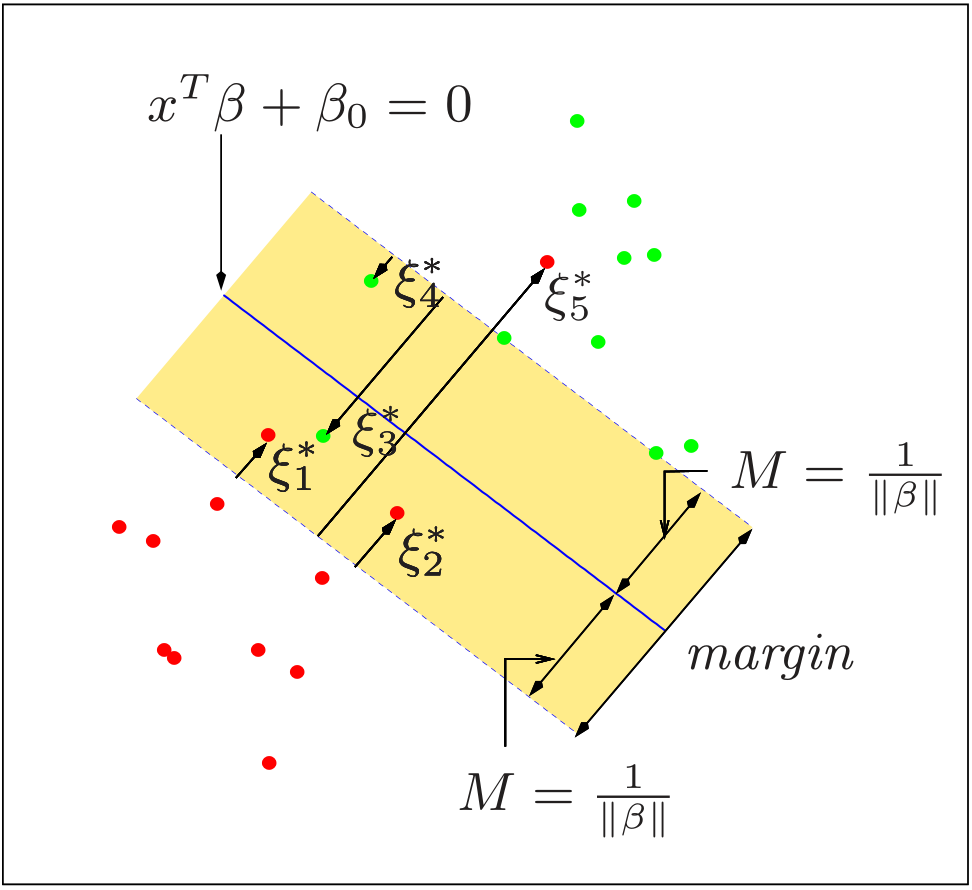
\includegraphics[width=0.4\linewidth]{sections/images/SVM.png}
    \caption{Support Vector Machine Illustration}
    \label{FigSVMIllustration}
\end{figure}

    Primal $ \theta _P $:
    \begin{equation*}
        \begin{aligned}
        \mathop{\arg\min}\limits_{\beta ,\beta _0:M=1/\Vert \beta  \Vert }\quad &\dfrac{1}{2}\Vert \beta  \Vert^2+C\sum_{i=1}^N\xi _i \\
        s.t.\quad & y_i(x_i'\beta +\beta _0)\geq 1-\xi _i&i=1,2,\ldots,N\\
        &\xi _i\geq 0&i=1,2,\ldots,N
        \end{aligned}
    \end{equation*}

    write the generalized lagrange function as defined in \autoref{EqaGeneralizedLagrangeFunction}:
\begin{align}
    \mathcal{L}(\beta ,\beta _0,\xi _i;\alpha ,\mu )=&\dfrac{1}{2}\Vert \beta  \Vert ^2+C\sum_{i=1}^N\xi _i+\sum_{i=1}^N\alpha _i\left[1-\xi _i-y_i(x_i'\beta +\beta _0)\right]-\sum_{i=1}^N\mu _i\xi _i \\
    s.t.\quad & \alpha _i\geq 0,\quad \mu _i\geq 0,\qquad i=1,2,\ldots,N
\end{align}
        
    dual problem is given when $ \dfrac{\partial^{} \mathcal{L}}{\partial \beta ,\beta _0,\xi _i^{}}=0 $:
\begin{align}
    \dfrac{\partial^{} \mathcal{L}}{\partial \beta ^{}}=0:\,&\hat{\beta }=\sum_{i=1}^N\alpha _iy_ix_i\\
    \dfrac{\partial^{} \mathcal{L}}{\partial \beta _0^{}}=0:\,&\sum_{i=1}^N\alpha _iy_i=0\\
    \dfrac{\partial^{} \mathcal{L}}{\partial \xi _i^{}}=0:\,&C=\alpha _i+\mu _i,\quad i=1,2,\ldots,N
\end{align}

    Dual $ \theta _D $:
\begin{align}\label{EqaDualProblemOfSVM}
    \theta _D(\alpha,\mu )=&\mathop{\min}\limits_{\beta ,\beta _0,\xi _i} \mathcal{L}=-\dfrac{1}{2}\sum_{i=1}^N\sum_{j=1}^N\alpha _i\alpha _jy_iy_jx_i'x_j+\sum_{i=1}^N\alpha _i\\
    s.t.\quad&0\leq \alpha _i\leq C\\
    &\sum_{i=1}^N\alpha _iy_i=0
\end{align}

    we can maximize $ \theta _D $ to obtain $ \hat{\alpha }_i $, $ \hat{\mu }_i=C-\hat{\alpha }_i $. And $ (\hat{\beta },\hat{\beta }_0,\xi _i) $ are given utilizing KKT condition for $ d^*=\mathop{\max}\limits_{\alpha ,\mu } \theta _D{\color{red}=}\mathop{\min}\limits_{\beta ,\beta _0,\xi _i}\theta _P=p^*  $:
\begin{align}
    &\hat{\alpha _i}\left[1-\hat{\xi }_i-y_i(x_i'\hat{\beta }+\hat{\beta }_0)\right]=0\\
    &(C-\hat{\alpha }_i)\hat{\xi }_i=0\\
    &1-\hat{\xi }_i-y_i(x_i'\hat{\beta }+\hat{\beta }_0)\leq 0\\
    &0\leq \hat{\alpha }_i\leq C\\
    &\hat{\xi }_i\geq 0\\
    &\hat{\beta }=\sum_{i=1}^N\hat{\alpha }_iy_ix_i
\end{align}

    discussion on different cases of $ \alpha _i,\xi _i $:
\begin{align}
    \hat{\alpha }_i=0:\,    &\hat{\xi }_i=0\\
    \hat{\alpha }_i=C:\,    &y_i(x_i\hat{\beta }+\hat{\beta }_0)=1-\hat{\xi }_i\\
    0<\hat{\alpha }_i<C:\,  &\hat{\xi }_0=0,\, y_i(x_i\hat{\beta }+\hat{\beta }_0)=1
\end{align}

    where all points $ \mathcal{I}^\mathrm{sv}:=  \{i^\mathrm{sv} \big|0<\hat{ \alpha }_{i^{\mathrm{sv} }}<C,\,\hat{\xi }_{i^\mathrm{sv} }=0 \} $ are called `\textbf{support vector}', that can be used to determine $ \beta _0 $:
\begin{align}
    \hat{\beta }=&\sum_{i=1}^N\hat{\alpha }_iy_ix_i=\sum_{i\in\mathcal{I}^\mathrm{sv} }\hat{\alpha }_iy_ix_i\\
    \hat{\beta }_0=&y_{i^\mathrm{sv} }-x_{i^\mathrm{sv} }'\hat{\beta }
\end{align}
    
\subsubsection{Support Vector Machine as Loss-Penalization Method}
    SVM Primal can be express in equivalent form with $ f(x_i) $ as prediction function, e.g. $ f(x_i)=\beta _0+x_i'\beta  $ for linear SVM:
    \begin{align}
        \begin{cases}
            \xi _i\geq 0\\
            \xi _i\geq 1-y_if(x_i)
        \end{cases} \Rightarrow \xi _i\geq \max\{0,1-y_if(x_i)\}= [1-y_if(x_i)]_+
    \end{align}
    
    in which $ [\,\cdot\,]_+\equiv \max\{0,\,\cdot\,\} $ is hinge loss\index{Hinge Loss}:
    \[
        \mathop{\arg\min}\limits_{\beta ,\beta _0}\sum_{i=1}^N\left[1-y_if(x_i)\right]_++\dfrac{\lambda }{2}\Vert \beta  \Vert ^2,\qquad \lambda =\dfrac{1}{C} ,\quad f(x_i)=\beta _0+x_i'\beta 
    \]
    
    which is naturally in an $ \mathop{\arg\min}\limits_{f}\sum_{i=1}^N\mathcal{L}\left(x_i,y_i,f(x_i)\right)+\dfrac{\lambda }{2}\mathcal{P}(f(\,\cdot\,))  $ Loss+Penalty form.  








\subsubsection{Kernel Support Vector Machine}




\subsection{Feature Expansion and Kernel Methods}
    Motivation: Map the data point $ x\in \mathcal{X}(e.g.\,=\mathbb{R}^p) $ to another feature space $ \mathcal{F}(e.g.\,=\mathbb{R}^M) $ (not necessarily a linear transform, usually $ M>p $, or just proper to describe the features). The mapping function lies in a Hilbert space $ \mathcal{H} $ of function:
    \[
        h(\,\cdot\,)=\left(h_1(\,\cdot\,),h_2(\,\cdot\,),\ldots,h_M(\,\cdot\,)\right)'\in \mathcal{H}:\, \mathcal{X} \to \mathcal{F}
    \]
    
    and we can construct model in feature space.    
    
\subsubsection{Reproducing Kernel Hilbert Space and The Representer Theorem}

    Based on the idea of feature space, make a step forward: the key focus of model is actually `measuring space structure by similarity between points' rather than having to define a feature space. i.e. describe similarity by a bi-linear \textbf{Kernel Function}\index{Kernel Function} 
    \[
        K(x,x') \in \mathcal{X}\times \mathcal{X}\to \mathbb{R}
    \]

    In intuition for Kernel is an `inner product kernel'. The Kernel corresponds a kind of inner product structure on $ \mathcal{H} $, the kernel should satisfies the following properties:
\begin{enumerate}[topsep=2pt,itemsep=2pt]
    \item Semi-Positive Definition:
    \begin{align}
        \iint K(x,y)g(x)g(y)\,\mathrm{d}x\mathrm{d}y\geq 0,\quad \forall g(\,\cdot\,)
    \end{align}
    
    or an equivalent form:
    \begin{align}
        \sum_{i,j=1}^n K(x_i,x_j)a_ia_j\geq 0,\quad \forall \{x_i\}_{i=1}^m,\{a_i\}_{i=1}^n,\quad \forall n\in\mathbb{Z}^+ 
    \end{align}
    \item symmetry:
    \begin{align}
        K(x,y)=K(y,x) 
    \end{align}
\end{enumerate}



Eigenvalue $ \gamma _i $ and eigen function $ \phi _i(x) $ of Kernel:
\begin{align}
     \int_x K(x,y) \phi _i(y)\,\mathrm{d}y=\gamma _i\phi_i(x)
\end{align}

    In Hilbert space, the eigen functions are orthonormal:
    \begin{align}
         \left\langle \phi _i,\phi _j\right\rangle = \int _x\phi _i(x)\phi _j(x) \,\mathrm{d}x =\delta _{ij}
    \end{align}

    And Kernel $ K(x,y) $ could be represented from its eigen value and eigen function:
    \begin{align}
        K(x,y)=&\sum_{i}\gamma _i\phi _i(x)\phi _i(y)
        % =&\left\langle \sqrt[]{\gamma _i}\phi _i,\sqrt[]{\gamma _i}\phi _i\right\rangle 
    \end{align}

    which is Mercer's Thm.:\index{Mercer's Theorem} Semi-positive definite symmetric kernel could be expressed as an inner product form. Such a form is also called the kernel trick\index{Kernel Trick} because it usually avoid calculating inner product in high dimensional space.
    
\begin{point}
    Reproducing Kernel Hilbert Space (RKHS)\index{RKHS (Reproducing Kernel Hilbert Space)}
\end{point}

    Now use set $ \{\phi _i\} $ as the orthonormal base to form a Hilbert space $ \mathcal{H}_K=\mathrm{span}\{\phi _i\}  $ i.e. any function $ f\in\mathcal{H}_K $ could be expressed as expansion
    \begin{align}
        \mu (x)=\sum_{i} \mu _i\phi _i(x)
    \end{align}

    The inner product defined for this Hilbert space is\footnote{Hilbert space is complete linear space with inner product defined.}
    \begin{align}
        \left\langle \sum_{i}\mu _i\phi _i(x), \sum_{i}\nu _i\phi _i(x)\right\rangle _{\mathcal{H}_K} = \sum_{i}\dfrac{\mu _i\nu _i}{\gamma _i}
    \end{align}
    and norm induced by inner product
    \begin{align}
        \left\Vert f \right\Vert _{\mathcal{H}_K}=\sum_{i}\dfrac{f_i^2}{\gamma _i},\qquad f(x)=\sum_{i}f_i\phi _i(x)
    \end{align}
    
    
    
    Note: when $ x $ is fixed, $ f_x(y)= K(x,y) $ is a function of $ y $, and vice versa. Use the above expansion and inner product:
    \begin{align}
        K(x,y)=& \sum_{i}\gamma _i\phi _i(x)\phi _i(y)\\
        =&\sum_{i}\sqrt[]{\gamma _i}\phi _i(x)\sqrt[]{\gamma _i}\phi _i(y)\\
        =&\sum_{i}\dfrac{(\gamma _i\phi _i(x))(\gamma _i\phi _i(y))}{\gamma _i}\\
        =&\left\langle \sum_{i}\gamma _i\phi _i(x){\color{brown} \phi _i(\xi )},\sum_{i}\gamma _i\phi _i(y){\color{brown} \phi _i(\xi )} \right\rangle _{\mathcal{H}_K}\\
        =&\left\langle K(x,\xi ),K(\xi ,y) \right\rangle _{\mathcal{H}_K}
    \end{align}

        which is the reproducing property of Kernel $ K(\,\cdot\,,\,\cdot\,) $ and its corresponding Hilbert space $ \mathcal{H}_K $
    
\begin{point}
    Representer Thm. for RKHS
\end{point}

    With Kernel and its corresponding RKHS defined, we could write a optimization problem as loss+penalty form:
    \begin{align}\label{EqaLossPenaltyFormOfRKHS}
         \mathop{\arg\min}\limits_{f\in\mathcal{H}_K}\sum_{i=1}^N\mathcal{L}(y_i, f(x_i)) + \dfrac{\lambda }{2}\left\Vert f \right\Vert^2 _{\mathcal{H}_K}
    \end{align}

    Representer Thm.\index{Representer Theorem}: Solution to above optimization has a \textbf{finite}  form
    \begin{align}
        \hat{f}(x)=\sum_{i=1}^N\hat{\alpha }_iK(x,x_i) 
    \end{align}

    i.e. we can optimize over $ \{\hat{\alpha }_i\}_{i=1}^N $, instead of optimizing over $ \{f_i\}_{i=1}^{\infty} $.

    norm of $ \hat{f} $ is represented as 
    \begin{align}
        \left\Vert \hat{f} \right\Vert ^2 _{\mathcal{H}_K}=&\left\langle \sum_{i=1}^N\hat{\alpha }_iK(x,x_i),\sum_{i=1}^N\hat{\alpha }_iK(x,x_i) \right\rangle _{\mathcal{H}_K}\\
        =&\sum_{i=1}^N\sum_{j=1}^N\hat{\alpha }_i\hat{\alpha }_j K(x_i,x_j)
    \end{align}

    Optimization problem \autoref{EqaLossPenaltyFormOfRKHS} is parameterized by $ \{\hat{\alpha }_i\}_{i=1}^N $:
    \begin{align}\label{EqaLossPenaltyFormOfKernel}
        \mathop{\arg\min}\limits_{\{\hat{\alpha }_i\}_{i=1}^N\in \mathbb{R}^N}\sum_{i=1}^N\mathcal{L}(y_i, \sum_{j=1}^N\hat{\alpha }_jK(x_i,x_j)) + \dfrac{\lambda }{2}\sum_{i=1}^N\sum_{j=1}^N\hat{\alpha }_i\hat{\alpha }_j K(x_i,x_j)
    \end{align}

    Or written in matrix form $ y=(y_1,y_2,\ldots,y_N) $ $ \alpha =(\alpha _{1},\alpha _{2},\ldots,\alpha _{N})  $, $ K=\{K(x_i,x_j)\}_{i,j=1}^N $:
    \begin{align}
        \mathop{\arg\min}\limits_{\alpha \in \mathbb{R}^N}\sum_{i=1}^N\mathcal{L}(y, K\alpha ) + \dfrac{\lambda }{2}\alpha 'K\alpha 
    \end{align}

    Classification criterion
    \begin{align}
        \hat{f}(x) =\sum_{i=1}^N\hat{\alpha }_iK(x,x_i)
    \end{align}
    

\subsubsection{Useful Kernel}
    Some useful Kernel for numeric vector $ x $:
    \begin{itemize}[topsep=2pt,itemsep=0pt]
        \item Linear Kernel (identity):
        \begin{align}
            K(x,y):=\left\langle x,y \right\rangle 
        \end{align}        
        \item $ d^\mathrm{th}  $ Degree Polynomial Kernel\index{dth Degree Polynomial Kernel@$ d^\mathrm{th}  $ Degree Polynomial Kernel}
        \begin{align}
            K(x,y):=\left(1+\left\langle x,y \right\rangle \right)^d
        \end{align}
        \item Radical Base Function Kernel\index{RBF Kernel (Radical Base Function Kernel)}: 
        \begin{align}
            K(x,y):=\exp\left[ -\dfrac{\left\Vert x-y \right\Vert ^2}{\sigma ^2} \right] 
        \end{align}
        \item Sigmoid Kernel\index{Sigmoid Kernel}: 
        \begin{align}
            K(x,y)=\tanh\left(1+\left\langle x,y \right\rangle \right) 
        \end{align}
    \end{itemize}

    Note that \autoref{EqaLossPenaltyFormOfKernel} includes Kernel $ K(\,\cdot \,,\,\cdot \,) $ only, thus Kernel trick could be applied to various scenarios once we could define a proper Kernel. e.g. Substring Kernel for string sequence.


\subsubsection{Kernel Support Vector Machine}
    Replace the inner produce term in Dual problem of SVM \autoref{EqaDualProblemOfSVM} into Kernel function to obtain Kernel SVM:\index{KSVM (Kernel Support Vector Machine)}
    \begin{align}
         &\mathop{\arg\max}\limits_{\alpha  } \sum_{i=1}^N\alpha  _i-\dfrac{1}{2}\sum_{i=1}^N\sum_{j=1}^N\alpha  _i\alpha  _jy_iy_j K(x_i,x_j) \\
         &s.t.\, 0\leq \alpha _i\leq C,\qquad \sum_{i=1}^N\alpha _iy_i=0\\
         &\hat{f}(x)=\sum_{i\in\mathcal{I}^\mathrm{sv} }\alpha _iy_iK(x,x_i)
    \end{align}

    Or use the loss+penalization primmal form of SVM:
    \begin{align}
        \mathop{\arg\min}\limits_{\hat{\alpha } }&\sum_{i=1}^N\left[ 1-y_i\sum_{j=1}^N\hat{\alpha }_jK(x_i,x_j) \right]_++\dfrac{\lambda }{2}\sum_{i=1}^N\sum_{j=1}^N\hat{\alpha }_i\hat{\alpha }_jK(x_i,x_j),\quad \lambda =\dfrac{1}{C} \\
        \hat{y}(x)=&\begin{cases}
            1 &,\hat{f}(x)=\sum_{i=1}^N\hat{\alpha }_iK(x,x_i)\geq s\\
            -1&,\hat{f}(x)=\sum_{i=1}^N\hat{\alpha }_iK(x,x_i)<s
        \end{cases}
    \end{align}
    
    Note: Here $ \alpha _i $ and $ \hat{\alpha }_i $ are not the same set of number, but the optimization problems are the same (if $ \{K(x_i,x_j)\} $ is non-singular). 

\subsubsection{SMO Algorithm for Kernel SVM}
    
    
\subsubsection{Kernel Regression}
\begin{point}
    Kernel Regression with Squared Error Loss
\end{point}

     Recall linear regression with RS loss
     \begin{align}
        \mathop{\arg\min}\limits_{\beta_0,\beta  }\sum_{i=1}^N\left[ y_i-\beta _0-x_i'\beta  \right]^2+\dfrac{\lambda }{2}\left\Vert \beta \right\Vert^2_2
     \end{align}

     replace linear classification $ f(x)=\beta _0+x'\beta  $ into Kernel $ K\alpha  $:
     \begin{align}
        \mathop{\arg\min}\limits_{\hat{\alpha }}(y-K\hat{\alpha } )'(y-K\hat{\alpha } ) +\dfrac{\lambda }{2}\hat{\alpha } 'K\hat{\alpha } 
     \end{align}

     Solution is similar to ridge regression form:
     \begin{align}
        \hat{\alpha }=(K+\lambda I)^{-1}y 
     \end{align}     

\begin{point}
    Kernel Logistic Regression
\end{point}

    In logistic regression, the loss function is binomial deviance $ \log\left[1+e^{-yf(x)}\right] $
    \begin{align}
        \mathop{\arg\min}\limits_{\hat{\alpha } }&\sum_{i=1}^N\log \left[1+e^{y_i\sum_{j=1}^N\hat{\alpha }_jK(x_i,x_j)}\right]+\dfrac{\lambda }{2}\sum_{i=1}^N\sum_{j=1}^N  \hat{\alpha }_i\hat{\alpha }_jK(x_i,x_j)\\
        \hat{y}(x)=&\begin{cases}
            1 &,\hat{f}(x)=\sum_{i=1}^N\hat{\alpha }_iK(x,x_i)\geq s\\
            -1&,\hat{f}(x)=\sum_{i=1}^N\hat{\alpha }_iK(x,x_i)<s
        \end{cases}
    \end{align}
    

\subsection{Clustering}
    Clustering is an important scenario of unsupervised learning $ \mathcal{D}=\{x_i\}_{i=1}^N $, to cluster `similar' data points into the same group. 

\subsubsection{Proximity Matrix}
    For separation concern, we should first define some metric to measure similarity between data
    \begin{align}
        d_{ij}=D(x_i,x_j) 
    \end{align}
    common usage of distance measure see \autoref{SubSectionClusteringAnalysis}
    
    And form the proximity matrix\index{Proximity Matrix} $ W $:
    \begin{align}
    D=\{d_{ij}\}_{i,j=1}^N 
    \end{align}
    
    Usually some clustering algorithm would claim some properties:
\begin{itemize}[topsep=2pt,itemsep=0pt]
    \item Non-negative element and non-zero diagonal:
    \begin{align}
        d_{ij}\geq 0,\,\forall i,j.\qquad d_{ii}=0,\,\forall i 
    \end{align}
    \item Symmetry
    \begin{align}
        D=D^T 
    \end{align}
\end{itemize}

    Overall dissimilarity:
    \begin{align}
        \bar{D}=\dfrac{1}{N^2}\sum_{i=1}^N\sum_{j=1}^ND(x_i,x_j) 
    \end{align}

\begin{point}
    Optimizing Goal of Clustering
\end{point}

    With similarity/dissimilarity defined, clustering target could be expressed as maximizing within cluster scatter/ minimizing between cluster scatter, with respect to clustering group $ C(\, \cdot \, ) $
    \begin{align}
        \mathop{\arg\max}\limits_{C(\, \cdot \, )}\dfrac{1}{2}\sum_{k=1}^K\sum_{i:C(x_i)=k}\sum_{j:C(x_j)=k}D(x_i,x_j)\\
        \mathop{\arg\min}\limits_{C(\, \cdot \, )}\dfrac{1}{2}\sum_{k=1}^K\sum_{i:C(x_i)=k}\sum_{j:C(x_j)\neq k}D(x_i,x_j)
    \end{align}

    The two forms are equivalent due to a fixed sum:
    \begin{align}
        \dfrac{1}{2}\sum_{k=1}^K\sum_{i:C(x_i)=k}\sum_{j:C(x_j)=k}D(x_i,x_j)+\dfrac{1}{2}\sum_{k=1}^K\sum_{i:C(x_i)=k}\sum_{j:C(x_j)\neq k}D(x_i,x_j)=\dfrac{1}{2}\sum_{i=1}^N\sum_{j=1}^ND(x_i,x_j):=T=\mathrm{const}
    \end{align}

    Usually search for cluster assignment is based on iterative greedy descent search.
    
    Some frequently used clustering methods are included in \autoref{SubSectionClusteringAnalysis}
    \begin{itemize}[topsep=2pt,itemsep=0pt]
        \item Hierarchical Method
        \item $ K $-Means
        \item EM-Gaussian Mixture Model
        \item DBSCAN \& OPTICS Density Method
    \end{itemize}
    
    In this section, an extra model based on spectrum is introduced

\subsubsection{Spectrum Clustering}
    Express the dataset as a Graph $ \mathcal{G}=(\mathcal{V},\mathcal{E},\mathcal{W}) $, where $ \mathcal{V}=\{v_i\}_{i=1}^N $ for vertex, $ \mathcal{E}=\{e_{ij}\}_{i,j=1}^N $, $ \mathcal{W}=\{w_{ij}\}_{i,j=1}^N $ for edges and weights. In this case cluster is a graph partition problem.

\begin{point}
    Graph Laplacian \index{Graph Laplacian}
\end{point}

Some definition:

\begin{itemize}[topsep=2pt,itemsep=0pt]
    \item Degree of vertex:
    \begin{align}
        d_i=\sum_{j=1}^Nw_{ij} 
    \end{align}
    \item Degree matrix
    \begin{align}
        D=\mathrm{diag}\{d_1,d_2,\ldots ,d_N\} 
    \end{align}
    \item Unnormalized graph Laplacian:
    \begin{align}
        L:= D-W
    \end{align}

    is symmetric and semi-positive definite
    \begin{align}
        \xi 'L\xi =\sum_{i,j=1}^Nw_{ij}(\xi _i-\xi _j)^2\geq 0,\quad\forall \xi \in\mathbb{R}^N 
    \end{align}
    
\end{itemize}

    Spectrum is based on studying the eigen vector and eigen value of $ L $.
\begin{itemize}[topsep=2pt,itemsep=0pt]
    \item For any graph Laplacian $ \mathop{L}\limits_{m\times m}  $, $ \mathbf{1}_m $ is a eigen vector with eigen value $ 0 $
    \item In the case that $ \mathcal{G} $ is \textbf{not} fully connected, with $ K $ subgraph $ \mathcal{G}=\{\mathcal{G}_1,\mathcal{G}_2,\ldots,\mathcal{G}_K\} $, i.e. $ W $ and $ L $ could be written in diagonal form (usually need some row/column transformation)
    \begin{align}
        L=\begin{bmatrix}
        L_{1}&0&\ldots&0\\
        0&L_{2}&\ldots&0\\
        \vdots&\vdots&\ddots&\vdots\\
        0&0&\ldots&L_{K}\\
        \end{bmatrix} 
    \end{align}

    the multiplicity of eigen value $ 0 $ is $ K $, with each eigen vector as
    \begin{align}
         \mathbf{1}_{\mathcal{G}_k}=[\mathbb{I}(v_1\in \mathcal{G}_k),\ldots,\mathbb{I}(v_N)\in\mathcal{G}_k],\quad k=1,2,\ldots,K
    \end{align}
    \item In real world case, the graph could probably expressed as a small deviance from a graph with subgraph:
    \begin{align}
         L=\begin{bmatrix}
            L_{1}&0&\ldots&0\\
            0&L_{2}&\ldots&0\\
            \vdots&\vdots&\ddots&\vdots\\
            0&0&\ldots&L_{K}\\
            \end{bmatrix} +\mathop{N\times N}\limits_{\delta } 
    \end{align}
    
    where we would expect the smallest $ K $ eigen value $ 0=\lambda _1\leq \lambda _2\leq\ldots \leq \lambda _K $ corresponds to the $ K $ cluster we want.

     
\end{itemize}

\begin{algorithm}{Spectral Clustering}
    \begin{enumerate}[topsep=2pt,itemsep=2pt]
        \item Compute $ \mathop{L}\limits_{N\times N}  $
        \item Determine the $ K $ smallest eigen values $ 0=\lambda _1\leq \lambda _2\leq\ldots \leq \lambda _K $ with eigen vector $ u_i $, $ i=1,2,\ldots,K $
        \begin{align}
            U=&[u_1,u_2,\ldots,u_K]=\begin{bmatrix}
            u_{11}&u_{12}&\ldots&u_{1K}\\
            u_{21}&u_{22}&\ldots&u_{2K}\\
            \vdots&\vdots&\ddots&\vdots\\
            u_{N1}&u_{N2}&\ldots&u_{NK}\\
            \end{bmatrix} 
            =[z_1,z_2,\ldots,z_N]^T\\
            z_i=&[u_{i1},u_{i2},\ldots,u_{iK}]^T,\quad i=1,2,\ldots,N
        \end{align}
    
        \item Cluster $ \{z_i\}_{i=1}^N$ with e.g. $ K $-Means.
    \end{enumerate}
    
        
\end{algorithm}


    Choice of normalized graph Laplacian, would cause different cluster results:
\begin{itemize}[topsep=2pt,itemsep=0pt]
    \item Ratio Cut $ L=I-D^{-1}W $
    \begin{align}
        \mathop{\arg\min}\limits_{\{\mathcal{G}_1,\ldots,\mathcal{G}_K\}}\dfrac{1}{2}\sum_{i=1}^K\dfrac{\mathrm{Bet}(\mathcal{G}_i,\mathcal{G}_{i}^\complement)}{|\mathcal{G}_i|}  
    \end{align}
    \item Normalized Cut $ L=I-D^{-1/2}WD^{-1/2} $
    \begin{align}
        \mathop{\arg\min}\limits_{\{\mathcal{G}_1,\ldots,\mathcal{G}_K\}}\dfrac{1}{2}\sum_{i=1}^K\dfrac{\mathrm{Bet}(\mathcal{G}_i,\mathcal{G}_{i}^\complement)}{\sum_{i\in\mathcal{G}_i}\sum_{j\in\mathcal{G}}d_{ij}}  
    \end{align}
    
\end{itemize}

\subsection{Tree-Based Classification Model}
    Idea of tree: divide the space $ \mathcal{X} $ into grids $ R_m $ and assign prediction into the most frequent class
    \begin{align}
        \hat{f}(x\in R_m)=\mathop{\arg\max}\limits_{k} \sum_{x_i\in R_m}\mathbb{I}(y_i=k)
    \end{align}

    But such method is not practical in high dimensional due to curse of dimensionality. Nore practical method would be a greedy search, each step along one variable.

\subsubsection{Tree-Based Classification}

\begin{point}
    Branch Growing Process
\end{point}

    Grow branch on a node $  $

\begin{algorithm}{Classification Tree}
    In each branck growing on a node:
    \begin{enumerate}[topsep=2pt,itemsep=2pt]
        \item Look for a splitting variable $ x_j $ and split value $ s $:
        \begin{align}
            &\mathop{\arg\min}\limits_{j,s}\left[N_\mathrm{left} \mathrm{ImPu}(x_i\in R_\mathrm{left}(j,s) )+N_\mathrm{right} \mathrm{ImPu}(x_i\in R_\mathrm{right}(j,s) )  \right] \\
            &R_\mathrm{left}(j,s)=\{x:x_j\leq s\},\quad R_\mathrm{right}(j,x)=\{x:x_j>s\}   
        \end{align}
        
        useful impurity measure $ \mathrm{ImPu}(\{x\})  $ with $ p_k(X=\{x\})$ defined
        \begin{align}
            p_k(X)=\dfrac{\sum_{x\in X}\mathbb{I}(C(x)=k)}{|X|}
        \end{align}
        
        
        \begin{itemize}[topsep=2pt,itemsep=0pt]
            \item Misclassification rate
            \begin{align}
                1-\mathop{\max}\limits_{k} p_k 
            \end{align}
            \item Gini impurity\index{Gini Impurity}
            \begin{align}
                \sum_{k=1}^Kp_k(1-p_k)=\sum_{k=1}^K\sum_{k'\neq k}p_kp_{k'} 
            \end{align}
            
            Gini impurity with category weight $ \mathop{W_K}\limits_{K\times K}=\{w_{kk'}\}_{k,k'=1}^K  $
            \begin{align}
                \sum_{k=1}^K\sum_{k'\neq k}w_{kk'}p_kp_{k'} 
            \end{align}
            
            \item Entropy
            \begin{align}
                -\sum_{k=1}^Kp_k\log p_k 
            \end{align}
            
            
            
            
        \end{itemize}
        \item usually the process ends when 
        \begin{align}
            |\mathrm{node} |\leq \mathrm{const},\quad \forall \mathrm{node}  
        \end{align}
        
        \item Apply cost complexity pruning strategy
        \begin{align}
            C_\alpha (T) =\sum_{m=1}^{|T|}N_m\mathrm{ImPu}(R_m)+\alpha |T|
        \end{align}
        
        where $ T $ is tree, $ |T| $ for number of nodes in the tree.
        
    \end{enumerate}
    
        
    
\end{algorithm}
    

    Comment:
\begin{itemize}[topsep=2pt,itemsep=0pt]
    \item Tree methods is well-interpreted, especially similar to a natural desicion making process
    \item Handle non-linear classification pattern
    \item Unstable to data.
\end{itemize}

    Performance of tree classification could be largely improved with bagging method and boosting method.

\begin{figure}[H]
    \centering
    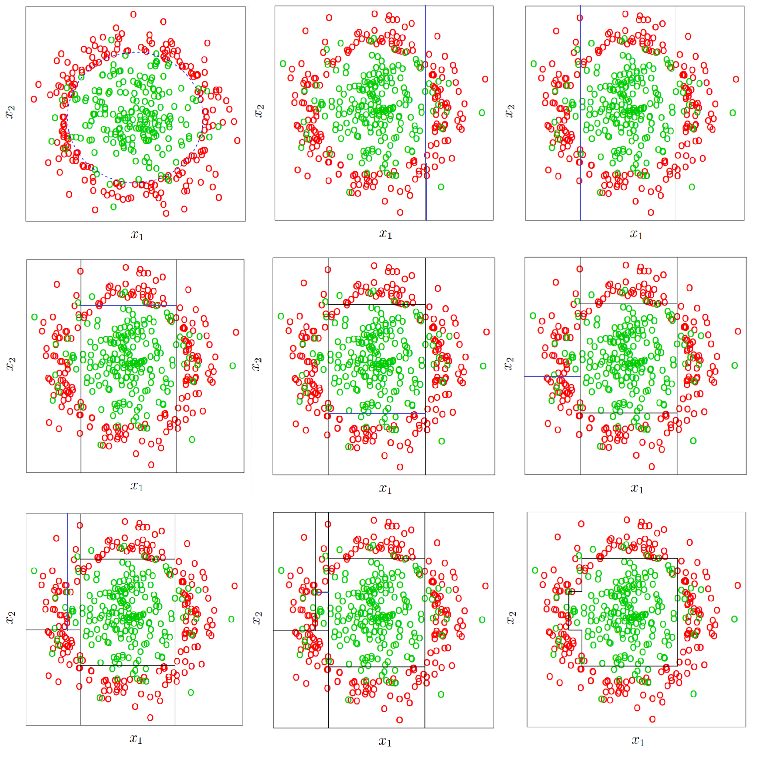
\includegraphics[width=0.8\linewidth]{sections/images/tree.png}
    \caption{}
    \label{}
\end{figure}


\subsubsection{Bagging and Boosting}
    
\begin{point}
    Bagging\index{Bagging Method (Bootstrap Aggregation Method)}\index{Bootstrap Aggregation}
\end{point}

    Bagging is short for \textbf{B}ootstrap \textbf{Ag}gregation. Idea: for $ B $ boostrapped training data, the boostrapping result
    \begin{align}
        \hat{f}_\mathrm{boot}(x)=\dfrac{1}{B}\sum_{b=1}^B\hat{f}_b(x)  \text{ or }=\mathop{\arg\max}\limits_{k} \sum_{b=1}^B\mathbb{I}(\hat{f}_b(x)=k)
    \end{align}

\begin{point}
    Random Forest\index{Random Forest}
\end{point}

    Random Forest aims at decorrelating trees to reduce variance when averaging trees.

\begin{algorithm}{Random Forest Bagging}
    \begin{enumerate}[topsep=2pt,itemsep=2pt]
        \item Generate $ B $ different boostrapped training data. (\textit{random 1} by bootstrap sampling)
        \item For each sample, grow a tree. In each split of tree (i.e. a branch growth), $ q\approx \sqrt[]{p} $ variable components are randomly selected for classification. (\textit{random 2} by randomizing components)
        \item Take average or vote of all $ B $ trees as the final result
    \end{enumerate}
    
    Comment: A prune is usually needed, cause variance is reduced by averaging.
        
\end{algorithm}
    
\begin{point}
    Boosting\index{Boosting Method}
\end{point}

    Idea: Fitting result of previous trees could be used to modify following trees. The error rate of each tree would influence the vote weight when bagging the results.
\index{Adaboost}

\begin{algorithm}{Adaboost}
    \begin{enumerate}[topsep=2pt,itemsep=2pt]
        \item Each observant is given weights $ w_i^{(0)}=\dfrac{1}{N},\,i=1,2,\ldots,N $
        \item For $ m=1:M $, $ M $ for loops of boosting:
        \begin{enumerate}[topsep=2pt,itemsep=2pt]
            \item Grow a tree $ T^{(m)}(x) $ with weight $ w_i^{(m)} $
            \item Compute \textbf{error rate}
            \begin{align}
                \mathrm{err}^{(t)} :=\dfrac{\sum_{i=1}^Nw_i^{(m)}\mathbb{I}(y_i\neq T^{(m)}(x_i))}{\sum_{i=1}^Nw_i^{(m)}}
            \end{align}

            and define 
            \begin{align}
                 \alpha ^{(m)}=\log\left[(1-\mathrm{err}^{(m)} )\big/\mathrm{err}^{(m)}\right]
            \end{align}
            \item Reset weights by
            \begin{align}
                w_i ^{(m+1)}=w^{(m)}\cdot\exp\left[ \alpha ^{(m)}\mathbb{I}(y_i\neq T^{(m)}(x_i)) \right]
            \end{align}
         
        \end{enumerate}
        \item Output
        \begin{align}
            \hat{f}(x)=\mathrm{sgn}\left[\sum_{m=1}^M\alpha ^{(m)}T^{(m)}(x)\right]  
        \end{align}
        
        
            
    \end{enumerate}
    
        
\end{algorithm}
    

\subsection{Neural Network}
\index{Neural Network}
\begin{point}
    Linear Perceptron with Activate Function\index{Linear Perceptron}\index{Activate Function}
\end{point}

    Usually linear perceptron is used as a neuron in neutral network:
    \begin{align}
        y=g(w_0+w_1x_1+\ldots+w_px_p) =g(x'w),\quad x_0\equiv 1
    \end{align}

    where $ g(\, \cdot \, ) $ is activate function. Such Perceptron could be optimized by gradient

    Some useful activate function:
\begin{itemize}[topsep=2pt,itemsep=0pt]
    \item Linear Threshold Unit (LTU)\index{LTU (Linear Threshold Unit)}\index{Activate Function!LTU (Linear Threshold Unit)}
    \begin{align}
        g(\xi )=\begin{cases}
            0,& \xi < 0\\
            1,& \xi \geq 0
        \end{cases} =\eta(\xi )
    \end{align}
    \item Logistic Function\index{Activate Function!Logistic Function}
    \begin{align}
        g(\xi )=\dfrac{1}{1+e^{-\xi } } 
    \end{align}
    \item Hyperbolic Tangent Function\index{Activate Function!Hyperbolic Tangent Function}
    \begin{align}
        g(\xi )=\tanh \xi =\dfrac{e^{2\xi }-1}{e^{2\xi }+1} 
    \end{align}
    \item Rectified Linear Unit (ReLU)\index{ReLU (Rectified Linear Unit)}\index{Activate Function!ReLU (Rectified Linear Unit)}
    \begin{align}
        g(\xi )= \begin{cases}
            0,& \xi < 0\\
            \xi ,& \xi \geq 0
        \end{cases}
    \end{align}
\end{itemize}

\begin{figure}[H]
    \centering
\def\layersep{2.5cm}
\begin{tikzpicture}[shorten >=1pt,->,draw=black!50, node distance=\layersep]
    \tikzstyle{every pin edge}=[<-,shorten <=1pt]
    \tikzstyle{neuron}=[circle,minimum size=12pt,draw=black,inner sep=0pt]
    \tikzstyle{input neuron}=[neuron];
    \tikzstyle{output neuron}=[neuron];
    \tikzstyle{hidden neuron}=[neuron];
    \tikzstyle{annot} = [align=left]

    % % Draw the input layer nodes
    % \foreach \name / \y in {1,...,4}
    % % This is the same as writing \foreach \name / \y in {1/1,2/2,3/3,4/4}
    %     \node[input neuron, pin=left:Input \#\y] (I-\name) at (0,-\y) {};

    \foreach \name / \x in {1,...,4}
        \node[neuron] (I-\name) at (-\x cm,-\layersep) {};
    \foreach \name / \x in {1,...,6}
        \path[xshift=1cm]
        node[neuron] (H-\name) at (-\x cm,0) {};
    \foreach \name / \x in {1,...,3}
        \path[xshift=-0.5cm]
        node[neuron] (O-\name) at (-\x cm,\layersep) {};
    \node[annot] (Error) at (-2.5 cm,2*\layersep) {$ \mathcal{L}=\dfrac{1}{2}\sum_{j=1}^l\left( \hat{y}_j-y_j \right)^2 $};
    \foreach \bg in {1,...,4}
        \foreach \ed in {1,...,6}
            \path (I-\bg) edge (H-\ed);
    \foreach \bg in {1,...,6}
        \foreach \ed in {1,...,3}
            \path (H-\bg) edge (O-\ed);
    \foreach \bg in {1,...,3}
        \path (O-\bg) edge (Error);
    
    \node[annot] at (I-1) {\small$ x_d $};
    \node[annot] at (H-1) {\small$ b_q $};
    \node[annot] at (O-1) {\small$ y_l $};


    \node[annot,right of=H-1, node distance=3.58cm] (hr) {$ \hat{b}_h=f(\sum_{i=1}^dv_{ih}x_i-\gamma  _h) ,\, h=1,\ldots,q$};
    \node[annot,right of=O-1, node distance=5.1cm] (or) {$ \hat{y}_j=f(\sum_{h=1}^qw_{hj}\hat{b}_h-\theta _j) ,\,j=1,\ldots,l $};
    \node[annot,right of=I-1, node distance=2.7cm] (ir) {$ x_i,\,i=1,\ldots,d $};
    \node[annot,left of=I-4, node distance=3cm] (il) {Input Layer};
    \node[annot,left of=H-6, node distance=2cm] (hl) {Hidden Layer};
    \node[annot,left of=O-3, node distance=3.5cm] (ol) {Output Layer};

    % % Draw the hidden layer nodes
    % \foreach \name / \y in {1,...,5}
    %     \path[yshift=0.5cm]
    %         node[hidden neuron] (H-\name) at (\layersep,-\y cm) {};

    % % Draw the output layer node
    % \node[output neuron,pin={[pin edge={->}]right:Output}, right of=H-3] (O) {};

    % % Connect every node in the input layer with every node in the
    % % hidden layer.
    % \foreach \source in {1,...,4}
    %     \foreach \dest in {1,...,5}
    %         \path (I-\source) edge (H-\dest);

    % % Connect every node in the hidden layer with the output layer
    % \foreach \source in {1,...,5}
    %     \path (H-\source) edge (O);

    % % Annotate the layers
    % \node[annot,above of=H-1, node distance=1cm] (hl) {Hidden layer};
    % \node[annot,left of=hl] {Input layer};
    % \node[annot,right of=hl] {Output layer};
\end{tikzpicture}

\caption{Structure of Feed-Forward Neural Network (1 Layer)}
\label{FigureMLP}
\end{figure}
    
    
    A MonoLayer perceptron with enough neurons (hidden units) could represent any coutinuous function. MultiLayer Perceptron (MLP)\index{MLP (MultiLayer Perceptron)} could even represent discontinuous functions. 
    
\subsubsection{Back Propagation}
    Perceptron system is usually optimized by back propagation (of gradient)\index{BP (Back Propagation)}.

    An example to optimize $ v_{ih},\,\gamma _h $ in \autoref{FigureMLP}:
    \begin{align}
        \dfrac{\partial^{} \mathcal{L}}{\partial v_{ih}}=&\sum_{j=1}^l\dfrac{\partial^{} \mathcal{L}}{\partial \hat{y}_j^{}}\dfrac{\partial^{} \hat{y}_j}{\partial \hat{b}_h^{}}\dfrac{\partial^{} \hat{b}_h}{\partial v_{ih}}\\
        =&\sum_{j=1}^l\hat{y}_j(\hat{y}_j-y_j)\cdot \dfrac{\partial^{} f(u)}{\partial u^{}}\Big|_{u=\sum w_{hj}\hat{b}_h-\theta _j}w_{hj}\cdot \dfrac{\partial^{} f(v)}{\partial v^{}}\Big|_{v=\sum_{i=1}^dv_{ih}x_i-\gamma _h}x_i\\
        \dfrac{\partial^{} \mathcal{L}}{\partial \gamma _h}=&\sum_{j=1}^l\dfrac{\partial^{} \mathcal{L}}{\partial \hat{y}_j^{}}\dfrac{\partial^{} \hat{y}_j}{\partial \hat{b}_h^{}}\dfrac{\partial^{} \hat{b}_h}{\partial \gamma _h}\\
        =&\sum_{j=1}^l\hat{y}_j(\hat{y}_j-y_j)\cdot \dfrac{\partial^{} f(u)}{\partial u^{}}\Big|_{u=\sum w_{hj}\hat{b}_h-\theta _j}w_{hj}\cdot \dfrac{\partial^{} f(v)}{\partial v^{}}\Big|_{v=\sum_{i=1}^dv_{ih}x_i-\gamma _h}\cdot (-1)
    \end{align}
    
    

